\documentclass[12pt]{article}
\usepackage[utf8]{inputenc}
\usepackage[brazil]{babel}
\usepackage{amsmath, amssymb}
\usepackage{graphicx}
\usepackage{indentfirst}
\setlength{\parindent}{1.25cm}
\usepackage{float}
\usepackage{hyperref}
\usepackage{geometry}
\usepackage{url}
\geometry{a4paper, top=3cm, bottom=2cm, left=3cm, right=2cm}
\usepackage{setspace}
\onehalfspacing
\usepackage{times} 
\usepackage{fancyhdr}
\usepackage{pdfpages}
\pagestyle{fancy}
\fancyhf{} % limpa os cabeçalhos
\fancyhead[R]{\thepage}
\renewcommand{\headrulewidth}{0pt}
\addto\captionsbrazil{\renewcommand{\listfigurename}{Lista de Ilustrações}}



\title{Reconhecimento Automático de Valores em Dados de RPG Utilizando Redes Neurais Convolucionais}
\author{Vinícius Silveira Bisinoto}
\date{Maio de 2025}

\begin{document}
\begin{titlepage}
    \centering
    \includegraphics[width=0.4\textwidth]{figuras/iftm.jpg}\par
    {\scshape\Large INSTITUTO FEDERAL DE EDUCAÇÃO, CIÊNCIA E TECNOLOGIA DO TRIÂNGULO MINEIRO \par}
    \vfill
    {\Large Vinícius Silveira Bisinoto\par}
    \vfill
    {\bfseries\Large Reconhecimento Automático de Valores em Dados de RPG Utilizando Redes Neurais Convolucionais\par}
    \vfill
    {\large UBERABA - MG\par}
    {\large 2025\par}
\end{titlepage}


\begin{titlepage}
    \centering
    {\Large Vinícius Silveira Bisinoto\par}
    \vspace{1.5cm}
    {\bfseries\Large Reconhecimento Automático de Valores em Dados de RPG Utilizando Redes Neurais Convolucionais\par}
    \vfill
    % Bloco justificado à direita
    \begin{flushright}
        \begin{minipage}{0.5\textwidth}
            Trabalho de Conclusão de Curso apresentado ao Instituto Federal de Educação, 
            Ciência e Tecnologia do Triângulo Mineiro, Campus Uberaba Parque Tecnológico, 
            como requisito parcial para a conclusão do Curso de Engenharia da Computação.\\
            Orientador: Prof. Dr. Marcelo da Silva Barreiro
        \end{minipage}
    \end{flushright}
    \vfill
    {\large UBERABA - MG\par}
    {\large2025\par}
\end{titlepage}
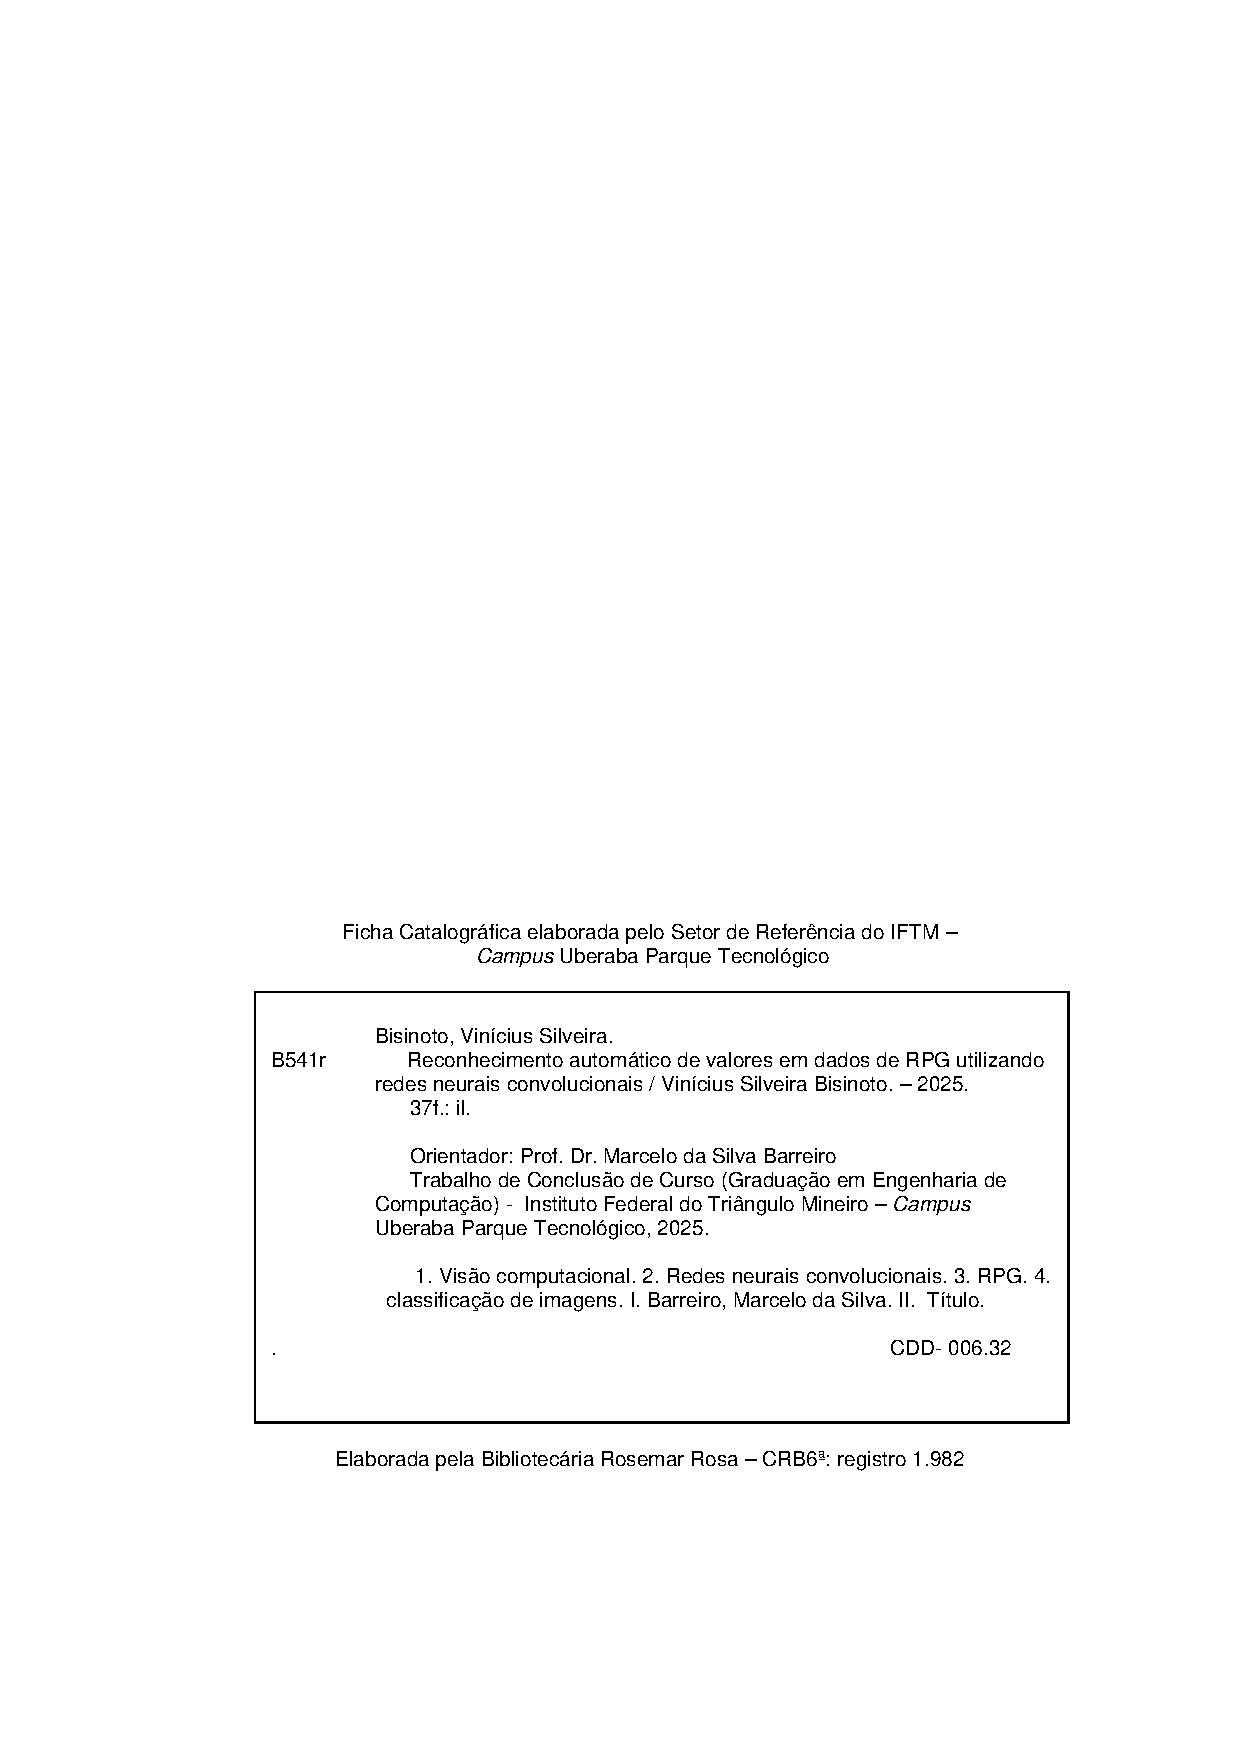
\includepdf{ficha.pdf}
\pagenumbering{gobble}
\begin{center}
    \Large\textbf{Agradecimentos}
\end{center}

A conclusão deste trabalho não seria possível sem o apoio, a presença e a força de diversas pessoas que estiveram ao meu lado ao longo de toda 
a jornada. Agradeço, antes de tudo, aos meus pais, \textbf{Germano} e \textbf{Valéria}, por todo o suporte incondicional oferecido ao 
longo deste processo. Em um período especialmente difícil da minha vida, vocês foram o alicerce que me sustentou. Sou profundamente 
grato pelo carinho, pela paciência e pela confiança que sempre depositaram em mim. Minha gratidão também à minha psicóloga, \textbf{Maíla}, 
por me ajudar a reencontrar equilíbrio e clareza em momentos em que a mente parecia um campo nebuloso. Sua escuta, sua orientação e seu 
trabalho foram essenciais para que eu conseguisse avançar e concluir este projeto. Agradeço à fotógrafa \textbf{Danielly},
 pela colaboração fundamental na produção das imagens utilizadas neste trabalho. Seu cuidado e profissionalismo deram vida à base visual 
 sobre a qual tudo foi construído. Expresso ainda meu carinho e gratidão a todos os meus amigos e companheiros de \textit{RPG}, 
 que fizeram — e continuam fazendo — parte da minha trajetória como mestre. Foram incontáveis histórias, mesas, risos e aventuras 
 compartilhadas que não só inspiraram este trabalho, mas também tornaram meus finais de semana mais vivos e felizes. Por fim, agradeço com 
 todo meu coração à \textbf{Louise Machado}, por estar ao meu lado em cada passo desta caminhada. Seu apoio foi tanto acadêmico quanto
 emocional, e foi justamente essa presença constante, em momentos de glória e de sofrimento, que me deu forças para continuar. Este 
 trabalho também é seu.

A todos vocês, meu mais sincero obrigado.



\newpage

\begin{center}
    \Large\textbf{Resumo}
\end{center}

\noindent
Este trabalho apresenta o desenvolvimento de um sistema baseado em redes neurais convolucionais (CNNs) para 
reconhecer automaticamente valores em dados físicos de RPG a partir de imagens. Foram utilizadas técnicas 
de visão computacional, com foco em classificação multiclasse e pré-processamento de imagens. A arquitetura 
foi treinada com um conjunto próprio de imagens categorizadas. Os resultados obtidos demonstram a viabilidade 
da abordagem e sugerem possíveis aplicações em sessões híbridas ou automatizadas de RPG.

\vspace{0.5em}
\noindent
\textbf{Palavras-chave:} Visão computacional, redes neurais convolucionais, RPG, classificação de imagens.

\begin{center}
    \Large\textbf{Abstract}
\end{center}

\noindent
This work presents the development of a system based on convolutional neural networks (CNNs) to automatically 
recognize the values on the upper faces of physical RPG dice from images. Computer vision techniques were used, 
focusing on multiclass classification and image preprocessing. The architecture was trained on a custom-labeled 
image dataset. The obtained results demonstrate the viability of the approach and suggest possible applications 
in hybrid or automated RPG sessions.

\vspace{0.5em}
\noindent
\textbf{Keywords:} Computer vision, convolutional neural networks, RPG, image classification.
\newpage

\begin{center}
\listoffigures
\newpage
\section*{Lista de Siglas}
\begin{itemize}
    \item \textbf{RPG}: Role-Playing Game (Jogo de Interpretação de Papéis)
    \item \textbf{D\&D}: Dungeons and Dragons (Masmorras e Dragões)
    \item \textbf{d2, d4, d6, d8, d10, d12, d20}: Dados de RPG com 2, 4, 6, 8, 10, 12 e 20 lados
    \item \textbf{CNN}: Convolutional Neural Network (Rede Neural Convolucional)
    \item \textbf{OCR}: Optical Character Recognition (Reconhecimento Óptico de Caracteres)
    \item \textbf{XP}: Experience Points (Pontos de Experiência)
    \item \textbf{DM}: Dungeon Master (Mestre de Masmorra)
    \item \textbf{LARP}: Live Action Role-Playing (Jogo de Interpretação de Papéis ao Vivo)
    \item \textbf{MUDs}: Multi-User Dungeons (Masmorras Multijogador)
    \item \textbf{GURPS}: Generic Universal RolePlaying System (Sistema Genérico Universal de Interpretação de Papéis)
    \item \textbf{RNGs}: Random Number Generators (Geradores de Números Aleatórios)
    \item \textbf{PRNGs}: Pseudo-Random Number Generators (Geradores de Números Aleatórios Pseudo-Aleatórios)
    \item \textbf{GPUs}: Graphics Processing Units (Unidades de Processamento Gráfico)
    \item \textbf{3D, 2D}: Três Dimensões, Duas Dimensões
    \item \textbf{TCC}: Trabalho de Conclusão de Curso
    \item \textbf{RGB}: Red, Green, Blue (Vermelho, Verde, Azul)

    \item \textbf{ReLU}: Rectified Linear Unit (Unidade Linear Retificada)
    \item \textbf{OpenCV}: Open Source Computer Vision Library (Biblioteca de Visão Computacional de Código Aberto)
\end{itemize}

\newpage
\tableofcontents
\newpage
\end{center}


\pagenumbering{arabic}
\setcounter{page}{8}   
\section{Introdução}

Os jogos de interpretação de papéis (Role-Playing Games - RPGs) têm conquistado cada vez mais espaço não só 
como forma de entretenimento, mas também como ferramenta pedagógica, terapêutica e social. Desde o lançamento
de \textit{Dungeons \& Dragons} em 1974, o RPG se consolidou como um gênero de jogos que une imaginação, 
cooperação e raciocínio lógico, promovendo experiências imersivas onde os jogadores atuam em conjunto na 
construção de narrativas.  \cite{peterson2012playing,hitchens2007roleplaying}

Uma das características marcantes desses jogos é o uso de dados físicos para determinar sucessos ou fracassos
de determinadas ações, como ataques, testes de habilidade ou eventos aleatórios, e, diferentemente dos jogos 
de tabuleiro convencionais, o RPG utiliza-se de uma diversidade de dados poliédricos 
— como d4, d6, d8, d10, d12 e d20 — que ampliam a variação probabilística das ações dos jogadores e tornam 
o jogo mais dinâmico e imprevisível. Além de sua usabilidade, esses dados se tornaram símbolos da cultura 
RPGista, muitas vezes personalizados com diferentes materiais, cores e gravuras, ou até eternizados em tatuagens, 
obras artísticas e coleções, reforçando o vínculo afetivo entre jogador e dado.\cite{hitchens2007roleplaying}

Apesar do crescimento de plataformas digitais que oferecem alternativas de rolagem automatizada, como
\textit{Roll20} ou \textit{Foundry VTT}, e até comandos de rolagem em bots de Discord, muitos jogadores ainda
preferem o uso dos dados físicos. Essa preferência se deve tanto ao valor simbólico e afetivo atribuído aos
objetos quanto à percepção de que a aleatoriedade física é mais justa ou autêntica do que a gerada 
computacionalmente. O som do dado rolando, o toque, o peso e até o suspense visual da face superior prestes a 
ser revelada são elementos sensoriais que contribuem para a ambientação do jogo e tornam a experiência 
mais sensorial, orgânica e memorável. \cite{zagal2017role}

No entanto, essa escolha estética e emocional traz um desafio prático. Em sessões que envolvem múltiplas
rolagens com dados, que muitas vezes podem conter múltiplos dados simultâneos — como testes de dano, ataques 
em área ou ações conjuntas — a contagem manual dos resultados obtidos pode se tornar demorada e propensa a erros. 
Esse tempo de cálculo afeta diretamente o ritmo narrativo da partida, especialmente em jogos com muitos 
participantes ou quando os personagens utilizados estejam com suas habilidades já em maior nível, aumentando
os números e resultando que dezenas de dados acabem sendo lançados ao mesmo tempo. Mesmo entre grupos experientes, 
a perda de fluidez entre ação e contagem numérica pode comprometer a imersão da experiência e gerar frustrações.

A crescente demanda por ferramentas que otimizem o tempo de jogo sem abrir mão da experiência de rolagem física
motivou este trabalho, que propõe uma solução baseada em visão computacional para automatizar a leitura visual dos
dados físicos durante uma rolagem, mantendo o aspecto tradicional do RPG com os dados físicos enquanto melhora 
a fluidez narrativa das sessões através da velocidade que um cálculo automático pode trazer. 
\cite{szeliski2010computer,ibm_cnn,datacamp_cnn}

A Figura~\ref{fig:dados-rpg} ilustra alguns exemplos de dados utilizados em sistemas de RPG, destacando a
variedade de formatos e faces numéricas. Essa diversidade, embora enriqueça o jogo, representa também uma
dificuldade computacional para quem deseja automatizar a leitura desses elementos visuais.

\begin{figure}[H]
    \centering
    \includegraphics[width=0.8\textwidth]{figuras/rpg-dice.JPG}
    \caption[Exemplos de dados poliédricos utilizados em jogos de RPG.]{
    \centering
    Exemplos de dados poliédricos utilizados em jogos de RPG.\par
    \textit{Foto por Danielly Vitória Rodrigues, 2025.}}
    \label{fig:dados-rpg}
\end{figure}

Partindo deste contexto, este trabalho tem como objetivo analisar a viabilidade do uso de Redes Neurais 
Convolucionais (CNNs) para o reconhecimento automático dos valores presentes nas faces superiores 
de dados físicos utilizados em jogos de RPG, a partir de um banco de imagens previamente separado e 
categorizado conforme o valor exibido na face superior dos dados. 
A proposta envolve o desenvolvimento e a avaliação experimental de um modelo de classificação multiclasse 
baseado em técnicas de visão computacional e aprendizado profundo, com foco na análise de seu desempenho 
em condições práticas simuladas. Para isso, será utilizada uma arquitetura de Rede Neural Convolucional (CNN) 
composta por múltiplas camadas convolucionais e de \textit{pooling}, seguidas por camadas densas e uma camada de saída 
com função de ativação \textit{softmax}, adequada ao reconhecimento de múltiplas classes de saída — 
correspondentes aos valores possíveis nas faces dos dados de RPG. As CNNs foram escolhidas por demonstrarem
bastante eficiência em tarefas de reconhecimento de padrões visuais, especialmente em imagens onde existem 
cenários com variação de iluminação, ângulo, cor e textura. 
\cite{lecun1998gradient, goodfellow2016deep}

As Redes Neurais Convolucionais (CNNs) têm seu destaque em diversas áreas da inteligência artificial, como 
reconhecimento facial, diagnósticos por imagem, leitura de placas de veículos e OCR (Reconhecimento Óptico 
de Caracteres), sendo utilizadas amplamente devido ao seu sucesso em contextos que exigem robustez, 
acurácia e capacidade de generalização \cite{lecun1998gradient, goodfellow2016deep}. Por ter várias camadas 
organizadas em etapas, essa arquitetura consegue identificar detalhes visuais em diferentes níveis, o que a 
torna muito eficaz para reconhecer símbolos, números e formas em objetos tridimensionais. — como os dados 
físicos utilizados em jogos de RPG — mesmo sob condições variáveis de iluminação, ângulo ou resolução.

A principal motivação para o desenvolvimento deste estudo nasce da vivência pessoal do autor como mestre de RPG, 
especialmente ao observar, ao longo de diversas sessões, a forte preferência dos jogadores pelo uso de dados 
físicos. Mesmo com a ampla oferta de ferramentas digitais que simulam rolagens de forma prática e eficiente, 
é comum notar que muitos jogadores ainda optam pelos dados reais, seja pelo apego emocional, a sensação de adrenalina
e expectativa ao rolar um dado, ou pela conexão simbólica que esses objetos representam dentro da cultura do RPG.
No entanto, essa escolha, apesar de compreensível e até esperada, pode acabar trazendo desafios durante o jogo, 
principalmente em momentos em que múltiplos dados são rolados ao mesmo tempo. Nessas situações, a contagem 
manual dos resultados tende a consumir um tempo precioso, além de estar sujeita a erros que podem comprometer 
a precisão e, por consequência, a imersão e o ritmo narrativo da partida. Dessa forma, automatizar esse 
processo de leitura dos valores nos dados físicos surge como uma solução equilibrada: respeita e preserva a 
tradição dos jogos de mesa, mas aproveita os recursos da tecnologia para tornar a experiência mais fluida, 
dinâmica e eficiente para todos os participantes.

Essa proposta também se alinha com os avanços mais recentes no uso de sistemas de visão computacional, com 
destaque para o aumento da sua adesão em tecnologias assistivas. Um bom exemplo disso são os sistemas 
de reconhecimento óptico de caracteres (OCR), que hoje já são amplamente utilizados na conversão de documentos 
físicos em versões digitais editáveis, com uma precisão invejável. De forma semelhante, desenvolver um sistema 
capaz de identificar automaticamente os números presentes nas faces superiores dos dados físicos representa uma 
aplicação com potencial promissor. Tal recurso pode funcionar como uma importante ferramenta de apoio tanto para
mestres quanto para jogadores, especialmente para aquelas sessões realizadas de forma online ou híbrida, onde
a visualização e validação das rolagens físicas continua sendo valorizada como parte da experiência principal.

Com base nas necessidades identificadas ao longo da experiência prática com jogos de RPG de mesa, este trabalho 
tem como objetivo principal o desenvolvimento e a avaliação de um modelo computacional, fundamentado em redes 
neurais convolucionais (CNNs), capaz de reconhecer os valores exibidos nas faces superiores de dados físicos. 
Essa identificação será realizada a partir da análise de um conjunto de imagens previamente coletado e 
devidamente categorizado.

Para atingir esse objetivo, propõe-se então a execução das seguintes etapas:

\begin{itemize}
\item Construção de um banco de dados composto por imagens de diversos tipos de dados de RPG, capturadas sob 
diferentes ângulos de visão, exibindo valores diversos em sua face superior com o intuito de refletir a 
variabilidade presente em situações reais;
\item Projeção e treinamento de uma arquitetura de rede neural convolucional voltada especificamente para a 
tarefa de classificação multiclasse dos valores numéricos visíveis nas imagens;
\item  Avaliação do desempenho do modelo utilizando métricas quantitativas, como acurácia e taxa de erro, 
considerando diferentes cenários simulados;
\item Discussão voltada tanto à avaliação da aplicabilidade prática do sistema em sessões de RPG, quanto à 
identificação de pontos de melhoria e caminhos possíveis para o aprimoramento e a evolução do projeto em 
versões futuras.
\end{itemize}

A proposta citada parte, portanto, da oportunidade avaliada pela observação de uma limitação no uso dos dados 
físicos em sessões de RPG, propondo o uso de técnicas de aprendizado profundo como uma solução inovadora. 
Ao longo do trabalho, serão apresentados os fundamentos teóricos que embasam o projeto, a metodologia adotada para 
construção e validação do modelo, os resultados experimentais obtidos e, por fim, as considerações finais e 
sugestões para futuras melhorias.


\section{Fundamentação Teórica}

Este capítulo apresenta os fundamentos teóricos que sustentam o desenvolvimento do projeto, abrangendo os temas 
de jogos de RPG, visão computacional, aprendizado profundo, redes neurais convolucionais e reconhecimento de 
padrões visuais. O objetivo é fornecer ao leitor o embasamento necessário para compreender a relevância, os 
desafios e as soluções técnicas envolvidas no reconhecimento automático de valores em dados físicos de RPG.

\subsection{Jogos de Interpretação de Papéis (RPG)}

\subsubsection{História e Evolução dos RPGs}
Popularmente conhecidos como RPGs (do inglês Role-Playing Games), ou jogos de interpretação de papéis, são 
atividades que compõem uma das atividades lúdicas mais complexas e influentes da contemporaneidade popular. 
A origem dessa prática pode ser traçada a uma série de influências históricas, culturais e mecânicas ao longo 
do final do séc. XIX E XX culminando na criação do sistema formal de RPG: \textit{Dungeons \& Dragons} (D\&D), publicado 
no início da década de 70 por Gary Gygax e Dave Arneson. \cite{peterson2012playing, hitchens2007roleplaying}

Como consequência direta da evolução de jogos de guerra (\textit{wargames}) anteriormente praticadas por entusiastas 
militares, e civis, os RPGs não surgem de forma isolada. Esse predecessor era jogado com miniaturas, mapas e regras 
complexas que simulavam combates históricos e podem ser classificados como formas de recreação tática. diferentemente
desse estilo de jogo, Arneson, e logo depois Gygax, trouxeram uma grande inovação, com a substituição do controle de 
exércitos pelo controle de personagens individuais com papéis específicos e atributos únicos, com isso foi possível 
introduzir um elemento narrativo e subjetivo que diferenciou os RPGs dos jogos de tabuleiro e estratégia.
\cite{peterson2012playing}

Peterson\cite{peterson2012playing} também enfatiza os clubes de \textit{wargames} norte-americanos no desenvolvimento 
das primeiras versões do que se tornou o RPG moderno, com particularidade em \textbf{Blackmoor}, uma campanha criada por 
um dos co-criadores de \textit{Dungeons \& Dragons} como um teste, um dos primeiros mundos onde o jogador assumia um papel 
fixo e participava de aventuras cotidianas.

Com a publicação da primeira versão de \textit{Dungeons \& Dragons} houve a formalização dos RPGs como um gênero distinto ao 
introduzir conceitos centrais como atributos numéricos (Força, Destreza, sabedoria e etc.), rolagem de dados poliédricos 
(inicialmente apenas o d6), níveis de experiência (XP), classes (como guerreiro, mago ou paladino) e sistemas de combate 
que integravam chances aleatórias e uso de estratégia. Nesse jogo a proposta era simples: o mestre (ou \textit{Dungeon Master}, DM),
assumia o papel imparcial de arbitrar e narrar enquanto os jogadores os papéis de personagens fictícios que colaboram para 
a criação de uma história interativa e imersiva. \cite{witwer2018}

RPGs podem ser classificados em quatro categorias gerais\cite{hitchens2007roleplaying}: RPGs de mesa (como D\&D), RPGs ao vivo 
(Live Action Role-Playing Games, LARP), RPGs eletrônicos (Computer RPGs) e MUDs (Multi-User Dungeons). Essa classificação 
revela o tamanho da expansão do conceito de RPG para todo tipo de mídia e contexto diferente, porém mantém seu elemento 
principal sendo o de interpretação de um papel em um mundo imaginário ditado por regras.

Houve uma grande evolução estética e temática ao longo dos anos nos RPGs durante as décadas de 1980 e 1990 com o surgimento 
de sistemas alternativos como o GURPS (Generic Universal RolePlaying System), que dava liberdade para que os jogadores e o 
mestre aplicassem a ambientação que quisessem, Vampire: The Masquerade, que inaugurou o gênero Storyteller focado em 
interpretação, e Call of Cthulhu, baseado na obra de H. P. Lovecraft. com temática de horror. Com tramas que envolviam 
jogadores em interpretações dramáticas, dilemas morais e ambientações sombrias. Essas histórias ampliaram o alcance narrativo 
de um jogo inicialmente puramente estratégico.

A partir dos anos 2000, os RPGs sofrem uma grande popularização em nível global em decorrência do aumento de plataformas digitais, 
fóruns de discussões na internet e a ascensão de transmissões ao vivo por criadores de conteúdo além de podcasts especializados. 
Obras como Critical Role, Ordem Paranormal e o Nerdcast RPG levaram o RPG a uma nova geração de jogadores ao expandir a forma de 
entretenimento de forma extremamente interativa. \cite{correa2021}

A Figura~\ref{fig:rpg-evolucao} ilustra uma linha do tempo simplificada que representa a evolução dos RPGs, desde sua origem nos 
wargames até a contemporaneidade em plataformas digitais. De maneira geral, o RPG se consolida não apenas como ferramenta terapêutica, 
artística ou de entretenimento alternativo, mas educacional também.\cite{vieira2019}

\begin{figure}[H]
\centering
\includegraphics[height=0.85\textheight, keepaspectratio]{figuras/Linha_do_Tempo_RPG_Mundo.png}
\caption[Linha do tempo simplificada e ilustrada da evolução dos RPGs]{
\centering
Linha do tempo simplificada e ilustrada da evolução dos RPGs, desde os wargames até os RPGs modernos.\par
\textit{Fonte: Silva, Gabriela Prates da; Prates da Silva, Eduardo (2020). História do RPG: linha do tempo. 
figshare. Figure. \url{https://doi.org/10.6084/m9.figshare.12493895.v5}.}}
\label{fig:rpg-evolucao}
\end{figure}

\subsubsection{A Importância dos Dados Físicos no RPG}
Não há restrição quanto ao uso de dados nos jogos de roleplaying (RPG). Como disse Peterson (2012), o uso de dados para definir 
normas de jogo e garantir imersão de jogadores pode ser traçado até meados dos anos 60 no mundo dos jogos. Nos precursores dos 
RPGS modernos — os wargames — se fazia o uso do dado de seis lados comumente customizados e adaptados para aleatorizar chances de 
vitória ou vantagens entre os jogadores em batalhas. Dessa maneira, os dados tinham o papel de fundamentar a dinamicidade e 
influenciar de forma imparcial o desenrolar das partidas.

A customização e adaptação dos dados de seis lados durante a segunda metade do séc XX, até mesmo em espaços de jogos de roleplaying 
como D\&D, dava-se especialmente pela limitação dos dados baseados nos sólidos de Platão — como d4, d6, d8, d10 e o d20 — que apesar 
de garantirem uma aleatoriedade variada e promoverem aspectos mais complexos do jogo, não eram tão populares e nem tão facilmente 
encontrados. O custo se mantinha como a maior dificuldade: a fabricação de dados variados se restringia a empresas norte-americanas 
como a TSR e posteriormente a Wizards of the Coast, o que significava que qualquer jogador de outro país precisava importar os dados, 
dificultando o acesso a diferentes tipos. Mesmo assim, com a popularização global do hobbie, nos anos 2000, com o lançamento da 3ª 
edição de \textit{Dungeons \& Dragons} e pelo licenciamento aberto do sistema d20, surgiram fabricantes locais e maior acessibilidade 
aos dados poliédricos, reduzindo custos para jogadores de todo o mundo.

Com o seu apogeu no final dos anos noventa e início dos anos 2000, a popularidade de jogos de RPG teve uma certa 
queda ao longo dos anos. Segundo Peixoto e Albuquerque(2018): \cite{peixoto_albuquerque_2018}

\begin{quote}
\textit{“Um dos fatores possivelmente envolvidos em uma diminuição pelo interesse nos RPGs foi a popularização dos jogos digitais. 
Jogos digitais não exigem tanta leitura, nem tanta preparação por parte do mestre do jogo. Além disso, possibilitam que as 
pessoas joguem mesmo estando distantes, e oferecem grande riqueza nos recursos audiovisuais, na narrativa e na jogabilidade 
- o computador pode processar uma quantidade de regras que jogadores não conseguem processar em um RPG de mesa tradicional”}
\end{quote}


Com o distanciamento social e suspensões de encontros presenciais que a pandemia de Covid-19 trouxe, muitos grupos de 
jogos como os de RPG migraram para ambientes virtuais. A adaptação desse público para plataformas digitais 
de mesa virtuais se tornou uma alternativa viável, permitindo a continuidade do hobby, mesmo quando dados e materiais 
físicos não eram utilizados \cite{correa2021}. Ferramentas para rolagens virtuais como bots de Discord e simuladores 
integrados a essas mesas virtuais eram cada vez mais utilizadas para manter as campanhas ativas durante o isolamento, 
além de ampliar o acesso do RPG a novos públicos permitindo encontros de jogadores em diferentes locais.

Dados virtuais amplamente usados em jogos digitais, simulações, sistemas de sorteio e nas plataformas já citadas no 
parágrafo anterior, geralmente utilizam o mecanismo de geradores de números aleatórios (RNGs)\cite{ghiglieno2025geradores}. 
Idealmente, a saída de números aleatórios deve seguir princípios de uniformidade e independência, ou seja, esses números 
devem ser equiprováveis e independentes entre si. Porém, diferente do que o nome sugere, na maioria das vezes esses geradores 
utilizados nesse tipo de atividade não costumam produzir uma aleatoriedade verdadeira, sendo assim, de forma mais apropriada, 
podem ser chamados de geradores de números pseudoaleatórios (PRNGs). São rápidos, mas dependem de uma sequência de números 
previsível, com resultados capazes de serem antecipados. Nas plataformas ja citadas, como \textbf{Roll20}, esse é o tipo de 
gerador utilizado, uma vez que o tipo de atividade desempenhada requer rapidez nos resultados. Dessa maneira, o uso de dados 
e aleatorizadores virtuais garantem resultados não verdadeiramente aleatórios como dados físicos.

A Figura~\ref{fig:roll20-interface} apresenta a interface da plataforma \textbf{Roll20}. A interface inclui recursos para comunicação entre os participantes, gerenciamento 
do cenário e, principalmente, suporte a rolagens de dados virtuais, facilitando a continuidade das campanhas mesmo à distância. 

\begin{figure}[H]
\centering
\includegraphics[width=1.0\textwidth]{figuras/roll20-interface.png}
\caption[Interface da plataforma Roll20]{
\centering
Interface da plataforma Roll20.\par
\textit{Fonte: Imagem de divulgação oficial, disponível em: \url{https://roll20.net/}}
}
\label{fig:roll20-interface}
\end{figure}

Mesmo que essa adaptação para ambientes virtuais tenha ocorrido, garantindo assim a sobrevivência do RPG em momentos difíceis, 
a experiência presencial continua sendo a preferência entre os praticantes. Jogar com dados físicos pode oferecer benefícios 
únicos como aumentar a imersão dentro da narrativa ao criar tensão, contribuir para o estímulo do raciocínio lógico e matemático, 
especialmente em sistemas que exijam cálculos e modificadores \cite{vieira2019} e estimular interações sociais que favoreçam um 
senso de comunidade ao compartilhar dados.


\subsection{Visão Computacional}

\subsubsection{Definição e Objetivos}

Durante o desenvolvimento de sistemas que busquem compreender informações visuais do ambiente, a Visão Computacional 
se apresenta como uma área interdisciplinar da ciência e engenharia voltada justamente para essa tarefa. Com forte 
inspiração nos mecanismos da visão humana, essa área propõe o uso de algoritmos específicos e técnicas matemáticas 
como forma de possibilitar que máquinas consigam extrair padrões relevantes, interpretar imagens e tomar decisões 
com base em dados visuais capturados de câmeras ou vídeos.
\cite{szeliski2010computer}.

Dentro do escopo da Engenharia da Computação, o papel da Visão Computacional se destaca por funcionar como 
um ponto de interseção entre componentes de hardware e soluções de software, exigindo do profissional domínio 
técnico em áreas como álgebra linear, sinais e sistemas, inteligência artificial e arquitetura de computadores. 
A utilização de câmeras acopladas a sistemas embarcados, a implementação de paralelismo computacional com auxílio 
de GPUs e a aplicação prática de redes neurais convolucionais são exemplos que ilustram como essa área se insere 
nos pilares da formação em engenharia, dialogando com diversas camadas do conhecimento computacional.\cite{bishop2006pattern}

Os objetivos da Visão Computacional variam conforme o domínio de aplicação, mas incluem tarefas como:

\begin{itemize}
\item \textbf{Reconhecimento de padrões}: identificar rostos, placas de veículos, objetos ou caracteres;
\item \textbf{Segmentação de imagem}: separar regiões de interesse com base em características como cor, 
textura ou bordas;
\item \textbf{Rastreamento}: acompanhar o movimento de objetos ao longo do tempo em sequências de vídeo;
\item \textbf{Reconstrução tridimensional}: obter modelos 3D a partir de múltiplas imagens 2D;
\item \textbf{Análise de cenas}: compreender o contexto global de uma imagem, como a contagem de 
pessoas ou a detecção de anomalias.
\end{itemize}

O avanço das redes neurais convolucionais (CNNs), a disponibilidade de grandes conjuntos de dados rotulados 
e o aumento no poder computacional possibilitaram resultados significativos nos últimos anos, com aplicações 
em áreas como saúde (diagnóstico por imagem), indústria (inspeção automatizada), segurança (monitoramento 
por câmeras) e entretenimento (realidade aumentada).

Em projetos como este TCC, a Visão Computacional assume papel central, possibilitando a interface entre os 
dados físicos do mundo real (os dados de RPG) e o sistema computacional responsável por interpretá-los automaticamente.



\subsubsection{Etapas do Processamento de Imagens}

O processo de construção de um sistema de visão computacional envolve diversas etapas encadeadas, que vão desde 
a aquisição dos dados até a inferência dos resultados. Cada uma dessas etapas tem o seu papel no desempenho do modelo, 
exigindo que sejam feitas decisões técnicas pensadas com base nos objetivos do problema em questão.

A Figura~\ref{fig:cv-pipeline} ilustra o fluxo completo do trabalho em um sistema de visão computacional, trazendo 
destaque para os pontos de decisão e os vieses que podem influenciar negativamente o resultado final.

\begin{figure}[H]
\centering
\includegraphics[width=0.85\textwidth, height=0.35\textheight, keepaspectratio]{figuras/Computer-vision-pipeline.png}
\caption[Fluxo de um sistema de visão computacional]{
\centering
Fluxo de um sistema de visão computacional.\par
\textit{Fonte: Physics-Informed Computer Vision: A Review and Perspectives - Scientific Figure on ResearchGate.} \par
\raggedright
\textit{Available from: 
\href{https://www.researchgate.net/figure/Computer-vision-pipeline-showing-different-biases-and-different-points-of-physics_fig3_371136308}
{https://www.researchgate.net/figure/Computer-vision-pipeline-showing-different-biases-and-different-points-of-physics\_fig3\_371136308} 
[accessed 5 Jun 2025]}
}
\label{fig:cv-pipeline}
\end{figure}

Esse fluxo é composto por cinco etapas, sendo elas:

\begin{itemize}
    \item \textbf{Aquisição de dados}: A etapa onde ocorre a coleta das imagens ou vídeos que serão utilizados no 
    treinamento do modelo. Os dados podem vir de fotos (2 dimensões), sensores com profundidade (3 dimensões) ou 
    streamings em tempo real. A qualidade e a diversidade dos dados capturados influenciam diretamente a capacidade 
    do modelo de fazer generalização.

    \item \textbf{Pré-processamento}: A etapa na qual são aplicadas transformações que preparam os dados para serem 
    utilizados pela rede neural. Dentre as operações mais comuns estão conversão para tons de cinza, normalização 
    dos valores do pixels, e técnicas de aumento de dados (\textit{data augmentation}). No contexto deste trabalho, 
    essa etapa incluiu o corte das bordas, redimensionamento padronizado das imagens e conversão de canais de cor RGB.

    \item \textbf{Projeto do modelo}: A etapa responsável pela arquitetura da rede convolucional que será utilizada, 
    como o número de camadas, quais filtros, suas funções de ativação e dimensões de entrada/saída. Modelos populares, 
    como GoogLeNet, ResNet e Mask-RCNN, oferecem diferentes estratégias para resolver tarefas como classificação, 
    detecção ou segmentação.

    \item \textbf{Treinamento do modelo}: A etapa que o modelo é exposto às imagens rotuladas e ajusta seus pesos 
    internos utilizando funções de perda como a entropia cruzada (\textit{cross-entropy}) ou erro quadrático médio. 
    O desempenho do modelo é medido com base em sua acurácia e na capacidade de generalizar para dados não vistos.

    \item \textbf{Inferência}: A etapa após o treinamento. Aqui o modelo é utilizado para fazer previsões sobre novos dados. 
    O tipo de inferência pode variar entre classificação, segmentação, detecção de objetos ou regressão, dependendo 
    do objetivo do projeto.

\end{itemize}

Além das etapas técnicas, a imagem também destaca três tipos de vieses que podem afetar os resultados:
\textbf{viés de observação} (dados enviesados), \textbf{viés de aprendizado} (modelo limitado em sua capacidade de 
generalização) e \textbf{viés indutivo} (pressupostos errados no design do modelo).

O entendimento de todas essas etapas é essencial para engenheiros da computação que desejam aplicar visão computacional 
a problemas do mundo real, como o reconhecimento automático de valores em dados físicos de RPG proposto neste trabalho.

\subsection{Aprendizado de Máquina e Aprendizado Profundo}

\subsubsection{Conceitos Básicos de Aprendizado de Máquina}

O aprendizado de máquina, ou machine learning (ML), é uma área da inteligência artificial que se dedica ao desenvolvimento de algoritmos 
capazes de identificar padrões em dados e realizar previsões ou decisões com base neles, sem depender de regras fixas previamente 
programadas. Esse tipo de abordagem ganhou força nos últimos anos com a explosão da disponibilidade de dados e com o crescimento 
do poder computacional, consolidando-se como uma das tecnologias mais presentes no nosso cotidiano — desde sistemas de recomendação 
até diagnósticos médicos assistidos por computador. \cite{bishop2006pattern, goodfellow2016deep}

De forma geral, os algoritmos de aprendizado de máquina podem ser organizados em três categorias, dependendo do tipo de informação 
que o modelo recebe durante o treinamento:

\begin{itemize}
    \item \textbf{Aprendizado supervisionado:}  nesse modelo, o algoritmo treina com base em um conjunto de dados rotulado — ou seja, 
    cada entrada já vem acompanhada do resultado esperado. O objetivo é aprender a mapear as entradas para as saídas corretas, 
    minimizando os erros ao longo do tempo. Esse é o paradigma utilizado neste projeto, onde o modelo precisa aprender a reconhecer, 
    a partir das imagens dos dados físicos de RPG, qual valor numérico está visível na face superior.

    \item \textbf{Aprendizado não supervisionado:}  aqui, os dados não possuem rótulos. O foco é descobrir padrões ou estruturas ocultas 
    nos dados, como agrupamentos naturais (clustering) ou formas de reduzir sua dimensionalidade mantendo as informações mais relevantes. 
    Técnicas como k-means, PCA e DBSCAN são bastante comuns nesse cenário. \cite{bishop2006pattern}

    \item \textbf{Aprendizado por reforço:} esse tipo de abordagem envolve um agente que interage com um ambiente, recebendo recompensas ou 
    penalidades a cada ação. O objetivo é aprender, com o tempo, quais decisões levam aos melhores resultados acumulados. É muito aplicado 
    em jogos, robótica e problemas que envolvem decisões sequenciais. \cite{goodfellow2016deep}
\end{itemize}

A tarefa de classificação é um dos pilares do aprendizado supervisionado. Nela, o modelo precisa prever a qual classe uma determinada entrada 
pertence. Quando o conjunto de saídas possíveis é discreto, temos um problema clássico de classificação. Podemos subdividir esse tipo de 
tarefa em três casos principais:
\begin{itemize}
    \item \textbf{Classificação binária}: o modelo escolhe entre duas possibilidades — como em “é spam ou não é?”, ou “é um gato ou um cachorro?”.
    \item \textbf{Classificação multiclasse}: envolve três ou mais categorias que se excluem mutuamente. É exatamente o caso deste trabalho, em 
    que a rede precisa decidir entre oito valores possíveis (de 1 a 8) visíveis nas faces dos dados de RPG.
    \item \textbf{Classificação multilabel}: diferente do multiclasse, aqui uma mesma entrada pode se encaixar em mais de uma classe ao mesmo 
    tempo. É comum em sistemas que recomendam múltiplos gêneros de um filme, ou detectam vários objetos em uma única imagem.
\end{itemize}

Para avaliar o desempenho dos modelos de classificação, usamos métricas como acurácia, precisão, recall e F1-score. A qualidade dos dados de 
entrada — neste caso, as imagens — e a capacidade do modelo escolhido — como as redes neurais convolucionais — têm um impacto direto nos 
resultados que o sistema consegue entregar.

\subsection{Redes Neurais Convolucionais (CNNs)}

As Redes Neurais Convolucionais (\textit{Convolutional Neural Networks} – CNNs) são um tipo específico de rede neural desenvolvida para lidar 
com dados que apresentam estrutura espacial, como imagens. A grande vantagem dessas redes é sua capacidade de identificar automaticamente 
padrões visuais em diferentes níveis — como linhas, texturas e formas mais complexas — sem a necessidade de definir manualmente quais 
características o modelo deve procurar.

Isso fez com que as CNNs se tornassem o padrão de fato para tarefas de visão computacional, incluindo reconhecimento de objetos, 
análise de exames médicos por imagem e, como no caso deste projeto, o reconhecimento de valores numéricos em imagens reais de dados 
físicos de RPG. \cite{lecun1998gradient, goodfellow2016deep}

\subsubsection{Estrutura Geral de uma CNN}

Uma CNN é composta por uma sequência organizada de camadas que trabalham em conjunto para extrair e processar as informações visuais da 
imagem de entrada. De forma geral, os principais blocos que aparecem na maioria das arquiteturas são:

\begin{itemize}
    \item \textbf{Camadas convolucionais}: aplicam filtros (ou kernels) que percorrem a imagem e destacam padrões locais, como bordas ou curvas.
    \item \textbf{Camadas de pooling (ou subamostragem)}: reduzem a resolução da imagem, mantendo o que é mais importante e ajudando a
     evitar que a rede memorize detalhes irrelevantes.
    \item \textbf{Camada \textit{Flatten}}: pega a saída tridimensional das etapas anteriores e transforma em um vetor linear para ser 
    tratado pelas próximas camadas.
    \item \textbf{Camadas densas}: conectam todos os neurônios entre si e fazem a parte final da classificação com base nas características 
    extraídas.
\end{itemize}

No modelo utilizado neste trabalho, a arquitetura segue esse padrão: três blocos convolucionais com pooling, seguidos por uma camada 
\textit{Flatten}, uma camada densa intermediária e, por fim, a camada de saída com ativação \textit{softmax}, responsável por prever o 
valor numérico entre oito opções (de 1 a 8), conforme o que aparece na face superior dos dados.

\subsubsection{Funcionamento das Camadas Convolucionais}

As camadas convolucionais são o coração da CNN. Nelas, pequenos filtros — geralmente de 3x3 ou 5x5 — percorrem a imagem aplicando uma 
operação chamada convolução, que nada mais é do que um produto escalar entre o filtro e a parte correspondente da imagem. O resultado 
forma um \textit{mapa de ativação} (\textit{feature map}), que mostra onde e com que intensidade aquele padrão aparece na imagem.

Três elementos definem o comportamento dessa operação:

\begin{itemize}
    \item \textbf{Filtro (ou kernel)}: é o conjunto de pesos que a rede aprende para detectar padrões específicos — como uma linha horizontal, 
    por exemplo.
    \item \textbf{Stride:} define quantos pixels o filtro avança a cada passo. Strides maiores reduzem o tamanho da saída.
    \item \textbf{Padding:} adiciona bordas à imagem para que o tamanho da saída seja preservado ou para evitar perder informações nas 
    extremidades.
\end{itemize}

Essas camadas são fundamentais para identificar padrões visuais em diferentes posições da imagem. Isso é crucial neste projeto, já que o 
valor visível em um dado pode estar deslocado, girado ou até com pequenas imperfeições na imagem. \cite{lecun1998gradient, datacamp_cnn}

\subsubsection{Pooling e Redução Dimensional}

Depois de identificar padrões locais, é comum reduzir a quantidade de informações com camadas de pooling. Isso serve tanto para diminuir a 
complexidade computacional quanto para tornar a rede mais robusta a variações pequenas nos dados.

Os métodos mais comuns são:

\begin{itemize}
    \item \textbf{Max pooling:} pega o maior valor dentro de uma região (o mais usado).
    \item \textbf{Average pooling:} calcula a média dos valores da região.
\end{itemize}

Com o pooling, a rede passa a focar apenas nas informações mais relevantes, descartando redundâncias. No contexto deste trabalho, isso ajuda 
a lidar com variações de ângulo, rotação ou iluminação nas fotos dos dados — condições bastante comuns em imagens capturadas no mundo real.

\subsubsection{Funções de Ativação e Camadas Densas}

Para que a rede possa lidar com padrões mais complexos, é necessário introduzir não-linearidade por meio das funções de ativação. As mais 
utilizadas são:

\begin{itemize}
    \item \textbf{ReLU (Rectified Linear Unit):} $\text{ReLU}(x) = \max(0, x)$, simples e eficiente, acelera o treinamento e evita saturações.
    \item \textbf{Sigmoid:} retorna valores entre 0 e 1, útil em saídas binárias.
    \item \textbf{Softmax:} transforma o vetor de saídas em uma distribuição de probabilidades — ideal para problemas de classificação 
    multiclasse.
\end{itemize}

Neste projeto, é de extrema importância a compreensão da função ReLU nas camadas intermediárias e da softmax na camada de saída, 
já que nosso objetivo é classificar cada imagem em uma entre oito categorias exclusivas — os valores possíveis visíveis nos dados de RPG. 
\cite{goodfellow2016deep}

\subsection{Aplicações Relacionadas: Reconhecimento de Dígitos e Objetos}

O reconhecimento visual de dígitos, símbolos e objetos físicos tem sido uma das frentes mais exploradas da visão computacional 
desde seus primórdios. A combinação de redes neurais convolucionais (CNNs) com técnicas de pré-processamento de imagens abriu 
novas possibilidades para tarefas antes fortemente dependentes de regras manuais e heurísticas rígidas. Essa evolução torna as 
CNNs ferramentas particularmente promissoras para problemas como o reconhecimento automático de valores em dados de RPG — um desafio 
que, embora recente em termos práticos, compartilha princípios fundamentais com casos clássicos da área.

\subsubsection{Caso Clássico: LeNet-5 e MNIST}

Um dos marcos históricos na área foi o desenvolvimento da LeNet-5, arquitetura proposta por LeCun et al. (1998), considerada pioneira 
no uso de CNNs para tarefas de reconhecimento visual \cite{lecun1998gradient}. Inicialmente concebida para interpretar números 
manuscritos em documentos bancários, essa rede foi aplicada com sucesso ao conjunto de dados MNIST — uma base padronizada contendo 
dígitos manuscritos em imagens de 28x28 pixels em tons de cinza.

A arquitetura da LeNet-5 é composta por camadas convolucionais intercaladas com camadas de pooling, seguidas por camadas totalmente 
conectadas e uma saída com função \textit{softmax}. Sua estrutura simples, mas eficaz, influenciou significativamente os modelos modernos, 
servindo de base conceitual para redes mais profundas e complexas. Apesar da limitação computacional da época, a LeNet-5 alcançou acurácia 
superior a 99\% na tarefa de classificação dos dígitos do MNIST, demonstrando a robustez das CNNs diante de variações de escrita, espessura 
e alinhamento.

O caso do MNIST é amplamente citado na literatura por reunir atributos que facilitam o estudo controlado de redes neurais: base de dados 
bem rotulada, problema objetivo, e dificuldade razoável. No entanto, a tarefa de reconhecer números em dados físicos de RPG adiciona 
obstáculos significativos, como base de dados não uniforme, pouco volume de dados para trabalho, perspectiva tridimensional e variações de design 
e cor entre diferentes modelos de dados. Ainda assim, os princípios empregados na LeNet-5 permanecem relevantes e inspiram abordagens mais sofisticadas 
para o problema em questão.

\subsubsection{Projetos Semelhantes}

Uma das propostas mais próximas do presente trabalho é descrita por Wimsatt et al. (2021)~\cite{wimsatt2021dice}, que apresenta um sistema 
de interpretação de dados de RPG utilizando redes neurais convolucionais (CNNs) treinadas com um conjunto de aproximadamente 16.000 imagens 
coletadas a partir do Kaggle. O objetivo principal do projeto era criar um classificador automatizado com precisão superior a 95\% para 
auxiliar na análise de “justiça” dos dados, ou seja, investigar a ocorrência de vieses em rolagens.

A abordagem adotada envolveu a padronização das imagens por meio de recorte de fundo e conversão para tons de cinza, seguidos do 
redimensionamento para 100×100 pixels. Após o pré-processamento, as imagens foram manualmente organizadas em diretórios separados 
por tipo de dado (d6, d8, d10, etc.) e posteriormente por valor da face visível. A rede utilizada incorporava camadas convolucionais, 
pooling, dropout e camadas densas, culminando em uma ativação \textit{softmax} com 20 saídas (para o d20, por exemplo). Foram testados 
entre três e cinco blocos convolucionais, com regularizações aplicadas para mitigar sobreajuste.

Apesar de os resultados numéricos relatados indicarem alta acurácia de validação — entre 95.12\% e 99.76\% — é importante destacar 
que os autores identificaram algumas limitações relevantes em sua base de dados, como o recorte inadequado em fundos de madeira e a 
ausência de faces específicas para certos dados (por exemplo, lados ausentes do d20).

\textbf{O presente trabalho se distingue academicamente em pontos fundamentais}:

\begin{itemize}
    \item \textbf{Aquisição original de imagens}: Enquanto o estudo de Wimsatt et al. utilizou uma base pré-existente e pública, 
    este trabalho baseou-se em um conjunto de imagens autorais, capturadas profissionalmente com iluminação e enquadramento controlados. 
    Isso assegura homogeneidade e validade experimental.
    
    \item \textbf{Foco na experiência do jogador}: O projeto atual visa não apenas classificar faces de dados, mas também dar um pontapé inicial
    nessa tecnologia até alcançar sessões de RPG presenciais, com o objetivo de minimizar a contagem manual durante múltiplas rolagens, sem 
    comprometer a experiência tradicional do jogo. A proposta não se limita à análise estatística de dados, mas foca em usabilidade prática.
    
    \item \textbf{Segmentação por valor numérico}: Ao invés de dividir os dados apenas por tipo físico (d6, d8, etc.), o presente 
    estudo organiza as imagens diretamente em pastas por valor de face visível, agrupando diferentes tipos de dados em uma única 
    classe (ex.: imagens de diferentes d6 e d8 mostrando o valor "5" são tratadas como uma única classe).
    
    \item \textbf{Redução de escopo baseada na qualidade da base}: Este projeto adota um escopo reduzido (valores de 1 a 8) após
    uma análise crítica da distribuição de amostras. A decisão metodológica de remover valores com baixa representatividade (como 0 e 9) 
    confere mais robustez ao treinamento e evita sobreajuste causado por classes com poucos exemplos — uma preocupação pouco abordada no 
    projeto anterior.
    
    \item \textbf{Adaptação de arquitetura e experimentação iterativa}: Diferente do trabalho anterior que aplica diretamente múltiplas 
    camadas convolucionais e dropout, aqui foi realizada uma série de experimentações, como data augmentation (descartado por queda de 
    acurácia), variações de \textit{learning rate} e análise de comportamento de validação conforme o número de épocas, que será apresentado
    no próximo capítulo. Essa abordagem iterativa e adaptativa permite uma melhor compreensão do comportamento do modelo e sua capacidade
    de generalização.
\end{itemize}

Por fim, o presente trabalho complementa a literatura existente ao aplicar técnicas de visão computacional em um contexto de RPG,
explorando a interseção entre tecnologia e jogos de tabuleiro. A proposta não apenas busca resolver um problema prático, mas também
contribui para o avanço do conhecimento na área, oferecendo insights sobre a aplicabilidade de CNNs em dados físicos e a experiência do jogador.

\subsection{Considerações Finais}

Este capítulo apresentou o embasamento teórico necessário para compreender os fundamentos técnicos que norteiam o desenvolvimento e as 
motivações presentes neste trabalho. Partindo da contextualização histórica dos jogos de RPG e a conexão com os dados, avançando pelas 
principais etapas da visão computacional, pelo funcionamento interno das redes convolucionais e pela aplicação dessas ferramentas em casos 
clássicos e recentes de reconhecimento de dígitos e objetos físicos.

Além de fundamentar a escolha metodológica que será detalhada no capítulo seguinte, esta discussão evidencia como o projeto se 
posiciona na fronteira entre pesquisa acadêmica e aplicação prática. A combinação de um problema real, um conjunto de dados original e 
métodos consolidados de aprendizado profundo sustenta o potencial técnico e inovador da proposta, cujo desenvolvimento será explorado 
no próximo capítulo.



\section{Metodologia }

Este capítulo descreve os métodos empregados no desenvolvimento do presente trabalho, 
com foco na estruturação do conjunto de dados, no processamento das imagens, no modelo de rede neural 
convolucional utilizado e nas estratégias de treinamento e validação do classificador. As decisões 
adotadas ao longo do processo são justificadas com base na realidade do projeto e nas limitaçães 
observadas durante a execução experimental.

\subsection{Coleta e Estruturação do Conjunto de Dados}
Para a realização dos testes, foi construído um conjunto de imagens próprio contendo fotografias de dados 
físicos utilizados em jogos de RPG. As imagens foram capturadas em estúdio fotográfico, com auxílio da
profissional Danielly Vitória Rodrigues, garantindo qualidade adequada de resolução, iluminação e enquadramento.

A figura~\ref{fig:image-counter} ilustra as quantidades de imagens coletadas para cada tipo de dado,
com um total de 1.124 imagens, distribuídas entre dados de 4, 6, e 8 e 10 lados.
\begin{figure}[H]
    \centering
    \includegraphics[width=0.45\textwidth]{figuras/image-counter.png}
    \caption[Distribuição do conjunto da base de imagens]{
        \centering
        Distribuição do conjunto de imagens coletadas, com contagem por tipo de dado. \par
        \textit{Fonte: Autoria própria.}}
    \label{fig:image-counter}
\end{figure}

As imagens foram organizadas em pastas segundo os valores visíveis nas faces superiores dos dados, 
totalizando inicialmente 10 classes: \textit{0\_zero} até \textit{9\_nine}. Cada uma dessas pastas 
continha subpastas correspondentes aos diferentes tipos de dados (ex.: d4, d6, d8, d10)\,. 
Essa estrutura permitiu manter a diversidade de formatos dentro de cada valor, simulando 
condições reais de uso.

Entretanto, durante a análise da distribuição dos dados, foi observado que as classes 
\textit{0\_zero} até \textit{9\_nine} possuíam um número significativamente inferior de 
imagens em relação às demais. Essa escassez comprometia a representatividade estatística 
e a robustez do treinamento, além de aumentar o risco de viés ou sobreajuste da rede.

Por essa razão, optou-se por restringir o escopo do modelo inicial às classes 
\textbf{1 a 8}, que apresentavam uma quantidade razoável de imagens (acima de 80 
amostras por classe no total). As classes excluídas foram mantidas como 
possibilidade para expansão futura do projeto, mediante a ampliação da base.

\subsection{Processamento de Imagens}

Todas as imagens passaram por uma etapa de pré-processamento com o objetivo de remover 
espaços em branco ao redor dos dados e padronizar o formato das entradas. O processamento incluiu:

\begin{itemize}
\item \textbf{Corte absoluto}: Remoção de bordas fixas nas extremidades superior, inferior, 
esquerda e direita da imagem, mantendo foco no dado centralizado;
\item \textbf{Redimensionamento}: Ajuste da imagem para dimensões fixas de 160x160 pixels, 
facilitando a entrada na rede convolucional;
\item \textbf{Conversão RGB}: Padronização do canal de cor para compatibilidade com bibliotecas 
de visão computacional;
\end{itemize}

Esse tratamento foi realizado utilizando a biblioteca OpenCV. As imagens processadas foram salvas 
em pastas separadas para treino e validação.
\subsection{Divisão em Treinamento e Validação}

Para cada uma das classes (1 a 8)\,, as imagens foram embaralhadas e divididas em 80\% para 
treinamento e 20\% para validação. A divisão foi feita com semente fixa para garantir 
reprodutibilidade. Devido ao tamanho limitado do dataset, optou-se por não subdividir o 
conjunto de validação em um conjunto adicional de teste. Essa decisão visa manter uma 
quantidade mínima de imagens por classe nas avaliaçães, evitando séries com menos de cinco amostras.

Para futuros trabalhos, recomenda-se a coleta de um novo conjunto independente de imagens para 
testes finais e validação cruzada do modelo.

\subsection{Arquitetura da Rede Neural Convolucional}

A arquitetura da Rede Neural Convolucional (CNN) utilizada neste trabalho foi projetada para equilibrar 
capacidade de extração de características e simplicidade estrutural, considerando a dimensão relativamente 
pequena do conjunto de dados e o objetivo de classificação multiclasse (valores de 1 a 8). A estrutura final consiste em:

\begin{itemize}
\item Uma camada de reescalonamento (Rescaling) que normaliza os valores dos pixels das imagens de entrada para o intervalo
[0,1], dividindo por 255. Essa etapa é essencial para acelerar a convergência durante o treinamento.
\item Três blocos compostos por:
    \begin{itemize}
        \item Uma camada Conv2D com filtros 3x3, ativação \textbf{ReLU} e preenchimento 'same', com 16, 32 e 64 filtros, respectivamente; 
        \item Uma camada \textit{MaxPooling2D} após cada convolução, reduzindo as dimensões espaciais e promovendo generalização.
    \end{itemize}
\item Uma camada de \textit{Flatten}, que transforma o mapa de características extraído em um vetor unidimensional.
\item Uma camada densa \texttt{Dense}  com 128 neurônios e ativação \textbf{ReLU}, responsável por combinar as características extraídas.
\item Uma camada de saída \textit{Dense} com 8 neurônios e ativação \textbf{softmax}, adequada para classificação multiclasse com rótulos 
inteiros de 0 a 7 (associados às classes 1 a 8).
\end{itemize}

O modelo foi compilado com otimizador Adam e função de perda \textit{Sparse Categorical Crossentropy}, uma vez que os rótulos são 
inteiros e não codificados em one-hot, utilizando o otimizador Adam com taxa de aprendizado \textbf{0.0006}. A métrica de avaliação 
escolhida foi a acurácia.

A Figura~\ref{fig:modelo-cnn} apresenta um diagrama ilustrativo inspirado na arquitetura LeNet-5, 
um dos modelos de redes neurais convolucionais mais clássicos, proposto por LeCun et al. (1998) para 
reconhecimento de dígitos manuscritos. Embora a estrutura exata da rede implementada neste trabalho difira em 
termos de parâmetros, profundidade e dimensionalidade das entradas, o diagrama é representativo do fluxo de 
processamento típico de uma CNN: camadas de convolução seguidas por subamostragem (pooling), camadas densas 
totalmente conectadas e uma camada final com função de ativação \textit{softmax} para classificação multiclasse.

\begin{figure}[H]
    \centering
    \includegraphics[width=0.9\textwidth]{figuras/CNN-architecture.png}
    \caption[Esquema conceitual da arquitetura da Le-Net-5]{
        \centering
        Esquema conceitual da arquitetura de uma CNN, inspirado na LeNet-5. \par
        \textit{Fonte: Adaptado de LeCun et al. (1998)}.
        }
    \label{fig:modelo-cnn}
\end{figure}


\subsection{Treinamento do Modelo e Desafios Encontrados}

O treinamento da rede neural convolucional (CNN) foi conduzido de forma iterativa, passando por 
diversas fases de ajuste de parâmetros, avaliação de desempenho e análise qualitativa dos resultados. 
O objetivo principal era obter um modelo capaz de classificar corretamente os valores nas faces 
superiores de dados físicos de RPG com alta acurácia e boa generalização.

Inicialmente, o modelo foi treinado por 20 épocas, com um \textit{learning rate} de $0.001$, 
sem aplicação de técnicas de \textit{data augmentation}. Essa primeira configuração foi escolhida 
por simplicidade e por estar alinhada com abordagens comuns na literatura introdutória de CNNs.
Apesar da acurácia de treino apresentar crescimento constante, a acurácia de validação mostrava 
valores baixos, sugerindo dificuldade de generalização do modelo.

Tentativas subsequentes foram feitas para aumentar a robustez do treinamento por meio de técnicas 
de aumento de dados. Utilizou-se uma camada de \textit{data augmentation} composta por rotações, 
espelhamentos e zoom aleatórios. No entanto, todos os testes com essa abordagem resultaram em queda 
expressiva de desempenho, com redução da acurácia de validação para menos da metade do valor 
anteriormente obtido. Tais alterações possivelmente introduziram variações que descaracterizaram 
os padrões dos números nas faces dos dados, prejudicando o aprendizado.

Também foram avaliadas estratégias de tratamento de imagem, como conversão para escala de cinza, 
equalização de histograma e aplicação de \textit{thresholding}. Embora visualmente eficazes em 
destacar o contraste entre o fundo branco e o dado, esses tratamentos acabaram por remover detalhes 
importantes dos números em certos casos. A perda de informação visual comprometeu a capacidade de 
discriminação do modelo, levando à decisão de manter as imagens em sua versão RGB original, apenas 
cortadas e redimensionadas para $160 \times 160$ pixels.

Para melhorar a capacidade de aprendizado, o número de épocas foi aumentado para 40 e, posteriormente, 
50. Com isso, a acurácia de treino superou os 90\%, mas a acurácia de validação permaneceu 
significativamente inferior. Essa discrepância levantou a hipótese de um desequilíbrio na divisão dos 
conjuntos. O conjunto de validação, com apenas 10\% das amostras (proporção 90/10), continha um número 
muito limitado de imagens por classe, o que impactava negativamente a avaliação do modelo.

A divisão foi então ajustada para 80/20 (treinamento/validação), o que resultou em melhoria 
expressiva. Em uma das execuções com 50 épocas, observou-se que a acurácia de validação estabilizava 
por volta da 40ª época, formando um platô. Por isso, optou-se por reduzir o número de épocas para 40.

Além disso, o \textit{learning rate} foi ajustado para $0.0006$, com o intuito de proporcionar um 
aprendizado mais estável e menos sujeito a oscilações abruptas nos pesos da rede. Essa configuração 
final resultou em uma acurácia de treinamento de aproximadamente 84\% e acurácia de validação de 72\%, 
com perda de validação (val\_loss) estabilizada em torno de 0.95, o que indica um bom nível de generalização 
para a tarefa de classificação de oito classes distintas (valores de 1 a 8).

\subsection{Resultados e Avaliação do Modelo}

Seguindo a estrutura previamente definida, o modelo final foi treinado ao longo de 40 épocas, utilizando a arquitetura convolucional 
descrita anteriormente. O conjunto de dados, após o processamento, totalizou 1.124 imagens distribuídas em 8 classes, correspondentes 
aos valores de 1 a 8. A divisão foi realizada de forma balanceada por classe, com 80\% das imagens destinadas ao treinamento (895 amostras) 
e 20\% à validação (179 amostras), utilizando embaralhamento fixo para garantir reprodutibilidade.

A avaliação do desempenho teve como métrica principal a acurácia. A função de perda escolhida foi a \textit{Sparse Categorical Crossentropy}, 
apropriada para problemas de classificação multiclasse com rótulos inteiros. Já o otimizador utilizado foi o Adam, com taxa de aprendizado 
ajustada para 0{,}0006, visando maior estabilidade no processo de aprendizagem.

A Figura~\ref{fig:accuracy-40-epochs} apresenta a evolução da acurácia durante as 40 épocas, tanto para os dados de treinamento
quanto de validação. Observa-se uma tendência de crescimento contínuo no desempenho sobre o conjunto de treinamento, enquanto a 
validação estabiliza a partir da 30ª época — indicando que o modelo atingiu um ponto de convergência satisfatório.

\begin{figure}[H]
\centering
\includegraphics[width=1\textwidth]{figuras/Accuracy40Epochs.png}
\caption[Evolução da acurácia durante o treinamento]{
\centering
Evolução da acurácia de treinamento e validação ao longo das épocas, indicando a progressiva capacidade de generalização do modelo. \par
\textit{Fonte: Autoria própria.}}
\label{fig:accuracy-40-epochs}
\end{figure}

Complementando a análise, a Figura~\ref{fig:loss-40-epochs} mostra a redução contínua da função de perda ao longo do treinamento. 
A perda sobre o conjunto de validação se estabilizou em torno de 0{,}95, sem apresentar variações abruptas ou tendência de crescimento, 
o que reforça a ausência de sobreajuste (\textit{overfitting}) significativo.

\begin{figure}[H]
\centering
\includegraphics[width=1\textwidth]{figuras/Loss40Epochs.png}
\caption[Evolução da perda durante o treinamento]{
\centering
Evolução da perda de treinamento e validação, evidenciando um comportamento estável do modelo e ausência de sobreajuste severo. \par
\textit{Fonte: Autoria própria.}}
\label{fig:loss-40-epochs}
\end{figure}

Ao final do treinamento, o modelo alcançou acurácia de aproximadamente 84\% no conjunto de treinamento e 72\% no conjunto de validação.
Esses resultados demonstram desempenho satisfatório, considerando a variedade visual presente nas imagens — com diferentes ângulos, 
condições de iluminação e estilos de dados — e as limitações impostas pelo tamanho reduzido da base.

Para uma análise mais detalhada, foi construída a matriz de confusão (Figura~\ref{fig:confusion-matrix}), que permite observar a 
distribuição dos acertos e erros por classe. Nota-se que o modelo obteve desempenho positivo na maior parte das classes, embora erros 
mais frequentes tenham ocorrido entre os dígitos 1 e 2, e entre 6 e 7 — provavelmente devido à similaridade visual desses números sob 
determinados ângulos ou em condições adversas de iluminação.

\begin{figure}[H]
\centering
\includegraphics[width=1\textwidth]{figuras/confusionMatrix40Epochs.png}
\caption[Matriz de confusão do modelo]{
\centering
Matriz de confusão do modelo treinado, evidenciando os acertos e erros por classe. \par
\textit{Fonte: Autoria própria.}}
\label{fig:confusion-matrix}
\end{figure}

Além da avaliação quantitativa, uma análise qualitativa foi conduzida com o intuito de observar a robustez do modelo frente a 
variações reais nas imagens. Em geral, os resultados foram consistentes, mesmo diante de mudanças moderadas de orientação ou iluminação. 
Contudo, algumas limitações ainda persistem em casos de oclusão parcial dos números, presença de reflexos ou baixo contraste entre os 
dígitos e o fundo do dado, o que dificulta a generalização.

\subsection{Considerações Finais}

Os experimentos realizados confirmam a viabilidade da aplicação de redes neurais convolucionais no reconhecimento automático de valores 
em dados físicos de RPG. A acurácia de 72\% obtida na validação, aliada à estabilidade do treinamento e à ausência de sobreajuste crítico, 
indica que o modelo conseguiu aprender padrões relevantes mesmo com uma base limitada.

A abordagem adotada seguiu um processo iterativo e fundamentado, com diversos ajustes ao longo do desenvolvimento. Destacam-se, 
nesse contexto, a importância de uma boa divisão dos dados, da escolha adequada da arquitetura e da rejeição de estratégias que 
não apresentaram resultados satisfatórios, como certos métodos de aumento de dados e pré-processamentos agressivos.

Para trabalhos futuros, algumas possibilidades promissoras incluem:
\begin{itemize}
\item A ampliação da base de dados, com maior número de imagens por classe e inserção de situações mais variadas, como ângulos 
extremos ou iluminação irregular;
\item A experimentação com modelos mais profundos ou baseados em \textit{transfer learning}, aproveitando redes pré-treinadas;
\item A integração de reconhecimento óptico de caracteres (OCR) com segmentação automática de múltiplos dados presentes na mesma 
imagem, visando aplicações práticas em sessões reais de jogo.
\end{itemize}

Dessa forma, o presente trabalho oferece uma contribuição relevante para o uso da visão computacional em jogos físicos, 
propondo uma solução funcional e passível de expansão para o reconhecimento automatizado de valores em dados multifacetados.
\input{resultados.tex}
\section{Conclusão}

O presente trabalho teve como objetivo principal investigar e implementar uma solução baseada em \textit{visão computacional} e 
\textit{redes neurais convolucionais} (CNNs) para o reconhecimento automático de valores em dados físicos utilizados em jogos de RPG. 
A proposta surgiu da observação de um problema recorrente nas sessões de jogo presenciais: o tempo e a atenção exigidos para interpretar 
e somar manualmente os resultados de múltiplas rolagens de dados, especialmente em momentos de ação intensa ou resolução de combate. 
Ao buscar uma alternativa tecnológica que respeitasse a experiência tátil e emocional associada ao uso dos dados físicos — em contraste 
com simuladores digitais —, o projeto propôs um meio-termo entre a tradição e a automação.

Para alcançar esse objetivo, foi construída uma base de imagens real, capturada em estúdio fotográfico, com dados reais e sob 
condições controladas de iluminação, foco e posicionamento. Esse cuidado na coleta garantiu imagens com boa qualidade visual, 
adequadas ao treinamento de um classificador baseado em CNN. Após análise da distribuição dos dados, foi decidido limitar o escopo 
inicial às classes de valores de 1 a 8, devido à baixa representatividade de imagens para os valores 0 e 9, assegurando um treinamento 
mais equilibrado e confiável.

Durante o desenvolvimento, foram adotadas práticas fundamentais da engenharia de software e da engenharia da computação: desde o 
uso de bibliotecas especializadas em processamento de imagem (OpenCV) até a modelagem e treinamento da rede convolucional com o 
framework TensorFlow/Keras. O pipeline de pré-processamento incluiu corte, redimensionamento e padronização das cores em RGB, buscando 
preservar ao máximo os elementos visuais relevantes ao reconhecimento dos dígitos nas faces dos dados.

O processo de treinamento passou por diferentes experimentações: inicialmente com 20 épocas, sem técnicas de aumento de dados, e 
posteriormente com ajustes progressivos — como aumento para 40 épocas, ajuste do \textit{learning rate} e reformulação da proporção 
entre os conjuntos de treino e validação. Testes com \textit{data augmentation} e filtros de tratamento como conversão para escala de 
cinza e equalização de histograma foram avaliados, mas não resultaram em melhorias. Ao contrário, tais técnicas acabaram degradando o 
desempenho do modelo, demonstrando que, neste contexto específico, a preservação da fidelidade visual das imagens originais foi essencial.

O modelo final alcançou uma acurácia de validação de aproximadamente 72\%, com uma taxa de acerto de 84\% no conjunto de treinamento, 
e uma curva de aprendizado estável, sem indícios fortes de sobreajuste. A análise por matriz de confusão revelou que o modelo soube 
generalizar bem os padrões dos dados, embora ainda apresente dificuldades pontuais em classes visualmente semelhantes.

Do ponto de vista acadêmico, o trabalho dialoga com projetos anteriores da literatura que utilizaram CNNs para reconhecimento de dígitos 
(como o clássico LeNet-5) e com aplicações específicas voltadas ao reconhecimento de dados de RPG. Diferencia-se, no entanto, por propor 
uma base real e própria, com foco explícito na aplicação prática durante sessões de jogo físicas, e não apenas na análise estatística de 
equilíbrio dos dados. Além disso, propõe um modelo leve, adaptável, sem dependência de datasets externos prontos como os encontrados no 
Kaggle, reforçando sua originalidade e aplicabilidade.

\subsection*{Perspectivas Futuras}

Embora os resultados obtidos sejam promissores, este trabalho representa uma etapa inicial. Diversas frentes de aprimoramento podem ser 
exploradas em trabalhos futuros:

\begin{itemize}
    \item \textbf{Ampliação do conjunto de dados}: Incluir os valores 0 e 9, bem como múltiplos modelos e cores de dados, para aumentar a 
    robustez e generalização do modelo. Também incluir dados de 12 e 20 lados, que são comuns em jogos de RPG.
    \item \textbf{Segmentação automática de múltiplos dados}: Evoluir de uma abordagem baseada em imagens isoladas para o reconhecimento 
    simultâneo de múltiplos dados em uma única imagem. Alcançando com isso a capacidade de calcular somas de rolagens de dados
    complexas, como as comuns em sistemas de combate de RPG.
    \item \textbf{Uso de modelos pré-treinados}: Explorar técnicas de \textit{transfer learning} com arquiteturas mais profundas, 
    como MobileNet ou ResNet, para melhorar ainda mais a acurácia em bases pequenas.
    \item \textbf{Integração com aplicação mobile}: Desenvolver um aplicativo móvel que utilize a câmera do dispositivo para capturar
    imagens dos dados em tempo real, processando-as e retornando os valores reconhecidos instantaneamente. Isso poderia ser feito com
    uma interface amigável, onde o usuário poderia apontar a câmera para os dados e receber os resultados de forma rápida e precisa.
\end{itemize}

\subsection*{Considerações Finais}

A execução deste projeto evidenciou como os conhecimentos teóricos de disciplinas fundamentais da engenharia da computação — como 
processamento de imagens, Inteligência artificial, estrutura de dados e programação orientada a objetos — podem se transformar em soluções 
aplicáveis a cenários reais, até mesmo em contextos lúdicos e culturais como os jogos de RPG.

Ao unir rigor técnico com criatividade, este trabalho se insere na fronteira entre o entretenimento e a ciência, propondo um caminho 
viável para aproximar a inteligência artificial da mesa de jogo, sem abrir mão da essência que torna os dados físicos tão marcantes para 
jogadores em todo o mundo.


\newpage

\bibliographystyle{abnt}
\bibliography{referencias}

\end{document}
